\chapter{Plasma  Control}
\label{Chap2}

This chapter summarizes some of the architectures for the Plasma Control Systems (PCS) existing in several tokamaks focused on the  Multi-threaded Application Real-Time executor (MARTe) framework.  The last part of this chapter addresses some basic concepts on state-space representation, linear dynamic systems and different feedback control techniques which will be widely used on the description of the carried out work showed on next chapters. 

\section{Overview of control systems}
The control of  plasma position, shape and current among other parameters is one of the essential engineering problems for present and future magnetic confinement devices. This chapter presents the real-time infrastructure used to implement plasma magnetic control and  some of the main reconstruction codes that are needed to achieve it. Real-time for fusion devices is principally focused on performing control and reconstruction algorithms, whether is for plasma position, current density, etc. on a software cycle, also known as sampling time, as short as possible so the  control loop acting on the  machine actuators can successfully take the plasma to the equilibrium, usually the real-time control cycles on some of the devices presented on this sections are on the order of  $\approx ~ 50~\mu s$ (\cite{Choi2018}, \cite{Felici2014} and ~\cite{Valcarcel2010}). The PCS deal with the overall control of  fusion devices being responsible also for the  plasma configuration and scenario algorithms \cite[Chapter~8]{PCS_2018}. Even thought this entire work mainly focuses on position and shape control it is also important to mention the relevance of density control for tokamak operation for the gas feeding feedback ~\cite{densityControl}. Industrial control systems in fusion devices like water cooling and power supply control usually are controlled outside the domain of the PCS. Currently different PCS's are used in  tokamaks around the world. In this chapter the "DIII-D-like" PCS, the Syst\'eme de Contr\^ole Distribu\'e (SCD) and MARTe will be introduced, this last one being of special interest due to its extensive utilization in this work, likewise this chapter presents an overview of the equilibrium codes  used for the reconstruction of plasma parameters used for the control of the  position, shape and plasma current among other parameters. The last part of this chapter recalls some basic concepts of Linear-Time Invariant systems and control system design which will be widely used in further chapters.


\subsection{DIII-D Plasma Control System}  

The DIII-D-like PCS is used in various fusion research facilities such as EAST (China), K-STAR (South Korea), NSTX (USA) and MAST (UK). Early documentation regarding the PCS in DIII-D\footnote{DIII-D is a D-shape tokamak operated by General Atomics in San Diego, California. } refers to digitalization of analog signals transmitted to a high speed processor executing a shape control algorithm and then writing the result to a digital to analog converter for driving the controlled systems. The real-time computer used allows to perform operations with vectors and matrices required for the plasma shape control algorithm \cite{DIIDcontrol}. Figure ~\ref{DIII1991} shows the block diagram of the DIII-D PCS 30 years ago.
\smallskip

\begin{figure}[htbp]
	\centering
	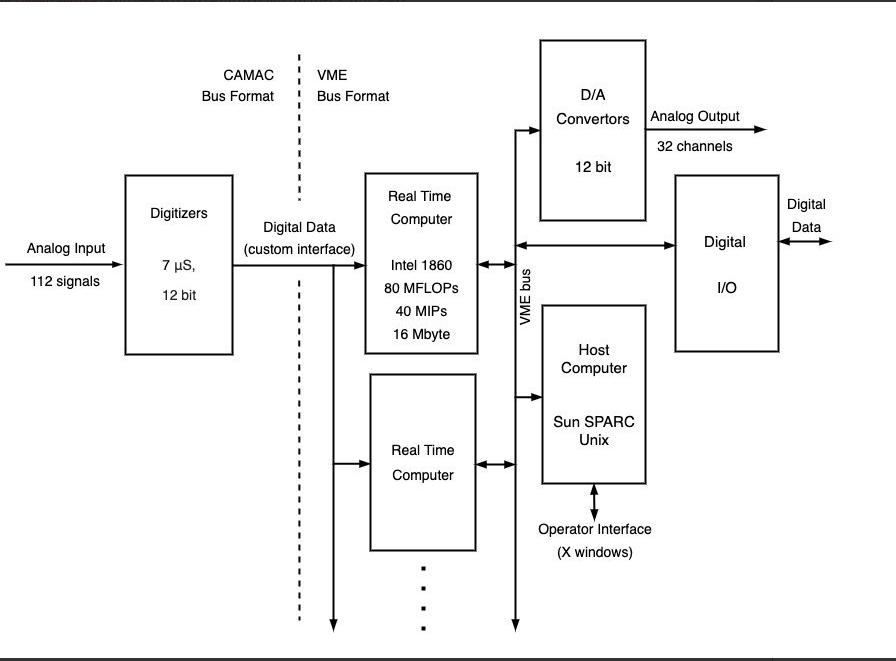
\includegraphics[width=0.65\textwidth]{Chp2/DIIDPCS_old.png}
	\caption{\label{DIII1991} DIII-D digital PCS in 1991 ~\cite{DIIDcontrol}.  }
\end{figure}

In recent years the DIII-D PCS had extensive software and hardware upgrades. The PCS present software consists of an infrastructure library core which provides all the routines that are necessary for implementing a basic and generic control system. The current  PCS hardware configuration uses a collection of  Intel Linux based multi-processor computers running in parallel to perform the real-time analysis and feedback control ~\cite{DIIID2013}. New digitalizers have been added to the real-time network to increase the number of signals acquired and to control hardware in real-time. Several real-time control algorithms were added and real-time data was added to external entities such as web server ~\cite{DIIIDnew}. In the current version of the PCS, a Myricom\footnote{Myricom networks also called Myrnet are high speed networking systems used to interconnect machines to form computer clusters. } network has been replaced with a 40 Gb/sec InfiniBand\footnote{InfiniBand is a network architecture from Mellanox designed to support I/O connectivity  and  reliability, availability, and serviceability Internet requirements ~\cite{MellanoxTechnologies2003}.  } network based on the Mellanox Connect-X 3\footnote{The Connect-X from the Mellanox company are Ethernet network interface cards with PCI Express.} hardware set. Figure ~\ref{DIIInew} shows the currently overall networking diagram of DIII-D PCS.


\begin{figure}[htbp]
	\centering
	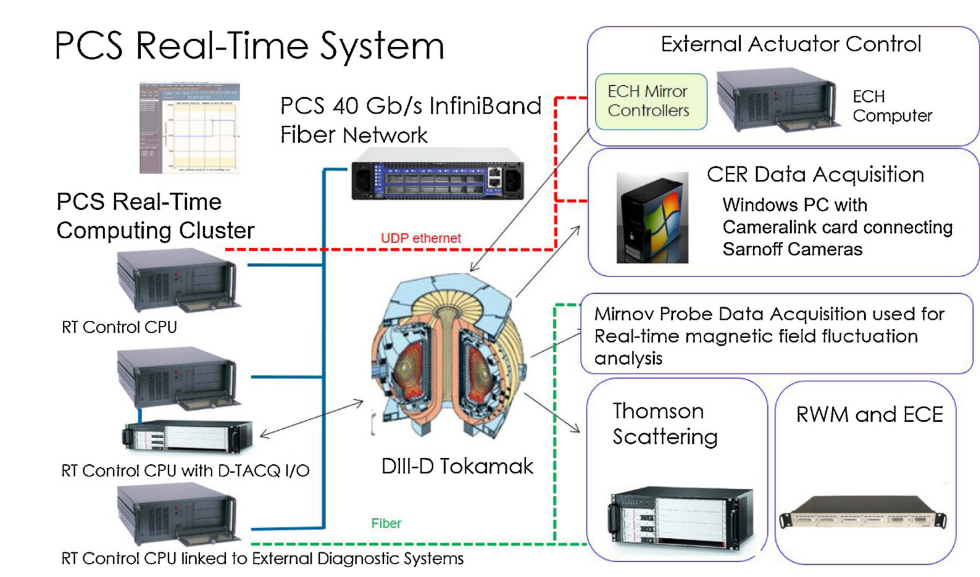
\includegraphics[width=0.65\textwidth]{Chp2/DIIIDPCSnew.PNG}
	\caption{\label{DIIInew} Actual DIII-D PCS real-time systems ~\cite{DIIIDnew}.  }
\end{figure}


\subsection{Syst\'eme de Contr\^ole Distribu\'e}

The TCV\footnote{The Tokamak \'a configuration variable (TCV) is  a medium size tokamak localized in Laussane,Switzerland. It is characterized by a highly elongated, rectangular vacuum vessel.} distributed control system uses a modular network of real time PC nodes linked by a real time network to provide feedback control over all of the actuator systems. Each node consists of a Linux PC either embedded on a Compact-PCI module or as a desktop computer with Intel CPU. A fiber optic ring network links the reflective memory (RFM) network cards in each node  \cite{TCVcntrl}.  The design of the diagnostic signal processing and control algorithms is performed in Matlab-Simulink software.  During the real-time execution  C/C++  code is generated from the Simulink and compiled  into a Linux shared library and distributed to target nodes  providing the input/output interface to the control algorithm code  ~\cite{TCVcntrl1}. Figure ~\ref{TCVcontrol} depicts the TCV SCD layout with the connectivity to diagnostics and actuators.


\begin{figure}[htbp]
	\centering
	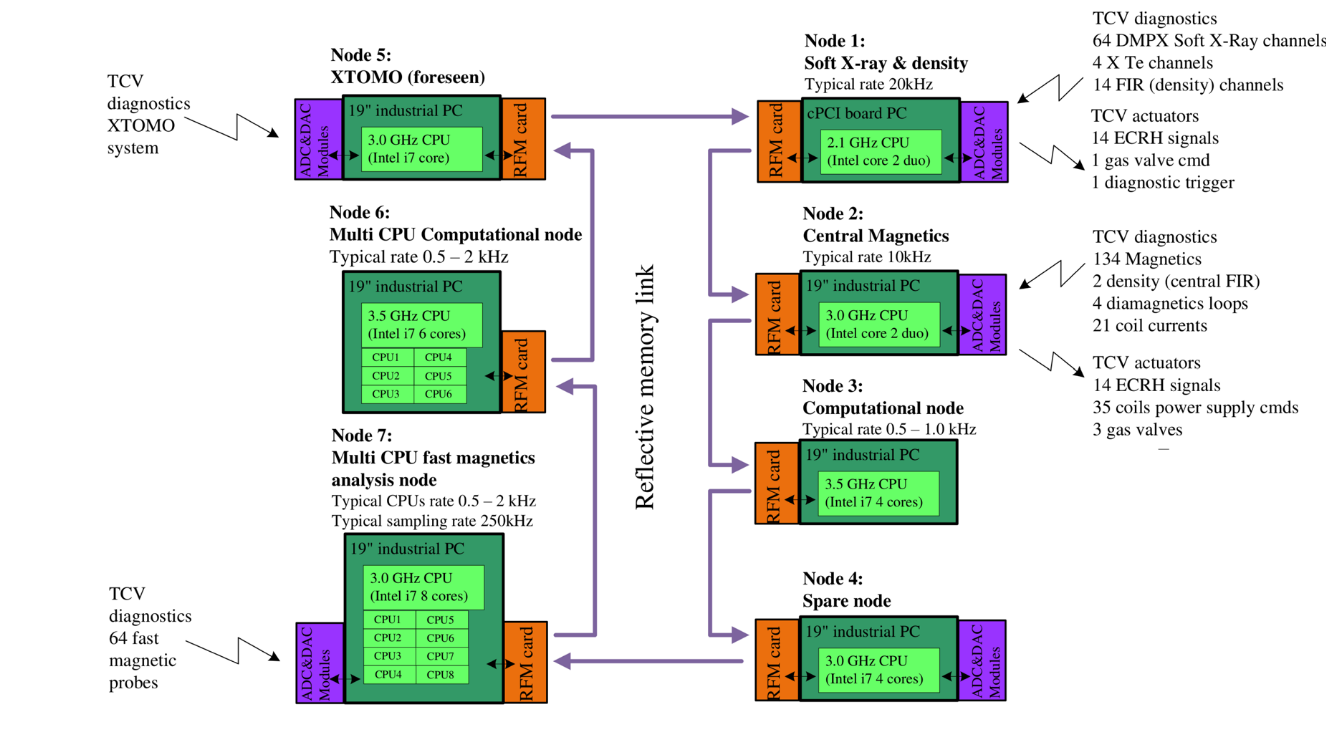
\includegraphics[width=0.65\textwidth]{Chp2/TCVcntrl1.png}
	\caption{\label{TCVcontrol} TCV SCD. Real-time network nodes connection. The nodes configurations 	are shown together with the typical diagnostic and actuator systems to which they are connected  ~\cite{TCVcntrl1}. This figure is missing the vertical stabilization controller that uses  Digital Signal Processors (DSP) system due to the higher control cycle speed of 5$~ \mu~s$ ~\cite{NunoPhD}. }
\end{figure}

\subsection{ASDEX Discharge Control System (DCS)}

The implemented control system existing on the ASDEX Upgrade  tokamak, the DCS  based on a modular software framework, supplies the functionality of  real-time diagnostic integration,  multivariable feedback schemes, actuator management,  monitoring and pulse supervision ~\cite{ASDEX2014}.\smallskip


 To distribute and parallelise the working load, part of the reconstructed  physical quantities are not computed by DCS but directly by real-time enabled digital diagnostic systems ~\cite{ASDEX2011}.  The DCS offers a user environment in the form of application processes (AP) holding the algorithmic part of control embedded in a framework infrastructure. Making use of the  polymorphic features of C++ the DCS  implements all infrastructure functions in base classes for the blocks, signals and other core component. The main components in DCS can be divided in function elements in the form of processes and DcsObjects, as well as data elements represented by signals, signal groups and parameters.  The hardware deployment of the DCS basically consists of a single-core 1 GHz PC with VxWorks operating system  and a multi-core 3.33 GHz PC running Concurrent Linux ~\cite{ASDEX2014}. Figure ~\ref{ASDEXcontrol} depicts the DCS control system function overview.  The blue boxes indicate the  sensor data sampling and measurement pre-processing, on magenta the control algorithms, the actuators on the red boxes and on the white boxes the references for the actuators and the segment scheduler which allows to select alternative sequences. 
 
 \begin{figure}[htbp]
 	\centering
 	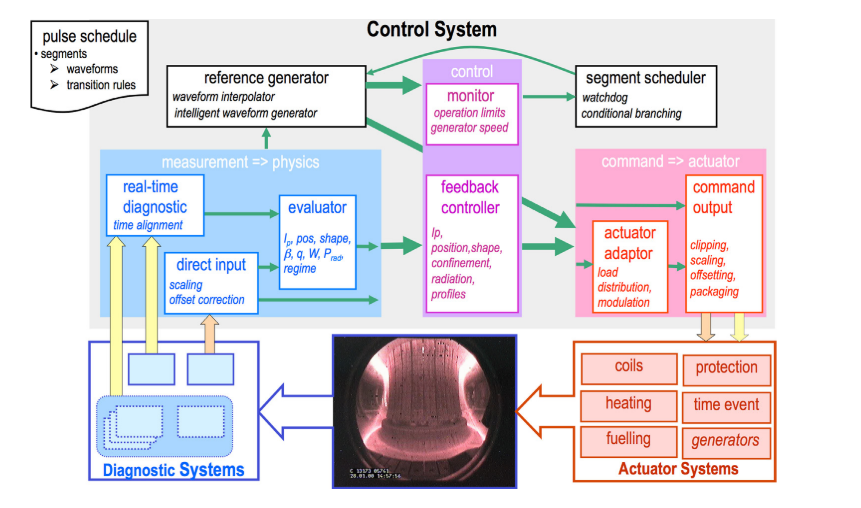
\includegraphics[width=0.75\textwidth]{Chp2/DCS_IPP.png}
 	\caption{DCS control system function overview. The blue boxes indicate the  sensor data sampling and measurement pre-processing, on magenta the control algorithms, the actuators on the red boxes and on the white boxes the references for the actuators and the segment scheduler which allows to select alternative sequences.   ~\cite{ASDEX2014}. \label{ASDEXcontrol}  }
 \end{figure}

\section{MARTe framework}

Regardless the nature of a real-time system, the design of it is usually related to the specific requirements it has, commonly this implies to have customized hardware and software which causes a lack in modularity and portability. When systems become bigger is convenient to provide a common library containing shareable functionalities and which also allows for modular implementations. In order to deal with this the MARTe framework was designed about a decade ago. MARTe was developed in order to standardize general real-time control systems for the execution of control algorithms and is based on a multiplatform $C^{++}$ library ~\cite{Neto2010},~\cite{JETRT}.  Previous implementations for a  software framework similar to MARTe were developed some years before for the JET tokamak. JETRT was a software framework used to develop real-time control and data acquisition systems which laid the foundation for current MARTe framework ~\cite{JETRT}. MARTe is currently used in several tokamaks such as JET, FTU, COMPASS and ISTTOK. 

  


\subsection{MARTe architecture }
The unitary MARTe component is the Generic Application Module (GAM). Each of the C++ programmed GAMs usually performs an specific task of the control system. The collection of interconnecting GAMs builds MARTe  \cite{Neto2011}. The GAMs  have an entry point to receive data driven configuration and a set of input and output channels to interface with other GAMs. The Dynamic Data Buffer (DDB) is a generic memory data bus where each GAM receives and produces data using DDB named channels. Usually each GAM is associated with a special function of the system like processing data of a specific diagnostic or perform some  control algorithm. MARTe hardware data interface and synchronization for inputs and outputs is performed using a special GAM called IOGAM. Figure ~\ref{GAMs} shows and xample of a set of GAMs connected to the DDB. Timing and hardware GAMs provide the I/O interface to the exterior, whereas a generic waveform GAM inputs the reference for a PID controller. Finally, the output is sent to a DAC and the data is stored for analysis by a collection GAM.  It should be noticed that the reference generation and the controller GAM are not aware of the changes in the data providers and data consumers.


\begin{figure}[htbp]
	\centering
	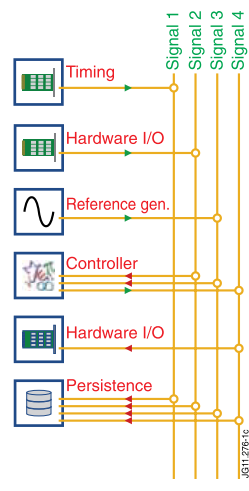
\includegraphics[width=0.35\textwidth]{Chp2/GAMs.png}
	\caption{\label{GAMs} MARTe GAMs structure using the DDB to exchange data in real-time.  \cite{MARTe2011}}
	
\end{figure}

\subsection{MARTe hardware containers}

This section describes the  hardware in-house developed at Instituto de Plasmas e Fus\~ao Nuclear (IPFN) for the use with the MARTe framework for the overall plasma control in different devices, specially the case for the JET, COMPASS and ISTTOK tokamaks. The devices presented in this thesis and used with the MARTe framework base their hardware on the  Advanced Telecommunications Computing Architecture (ATCA) standard, which is the most promising architecture to substantially enhance the performance and capability of existing standard systems as it is designed to handle tasks such as event building, feature extraction and high-level trigger processing ~\cite{ATCA2010}.\smallskip

At JET the data acquisition system for the vertical stabilization control is based on the PICMG 3.0 ATCA standard  and contains six data acquisition cards. Each board comprises 32 18-bit resolution analog-to-digital converters (ADC) acquiring at 2 Msamples/s. The cards are connected to the controller computer using the Peripheral Component Interconnect Express (PCIe) point-to-point links through the ATCA backplane ~\cite{Neto2010},~\cite{ATCA2006}. Data synchronization is performed in the master board, which is guaranteed by the firmware to be the latest to have data available. Once new data is available, it is collected and a new MARTe cycle starts. The CPU core isolation scheme allows to protect the real-time environment from spurious and undesired interrupt sources. Figure ~\ref{ATCa_JET} depicts a roughly JET scheme of the acquisition boards and its connection to the MARTe framework. The acquisition boards map in the controller computer memory a set of four buffers, the selected one is consecutively cycled every $50~ \mu s$  by the firmware. The first value written is the header and contains the absolute time since the last trigger, followed by the acquired  values of the ADCs, and finally by the footer containing the same value as the header. \smallskip

\begin{figure}[htbp]
	\centering
	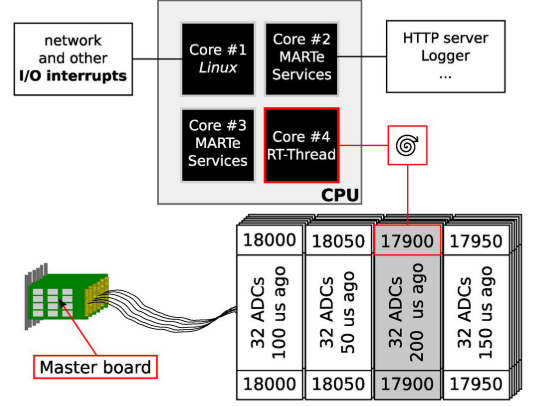
\includegraphics[width=0.55\textwidth]{Chp2/ATCA_JET.png}
	\caption{\label{ATCa_JET}  JET acquisition boards from the ATCA hardware  and its connection to the MARTe framework.  ~\cite{Neto2010}}
	
\end{figure}



The hardware used in the ISTTOK real-time control system is also  based on the ATCA standard while the old architecture was based on the Peripheral Component Interconnect (PCI) standard. It is worth to mention that the MARTe control cycle in ISTTOK is programmed to be of 100 $\mu s$, this value was calculated taking into account the time that each GAM takes to run. The ATCA acquisition boards are composed by 32  ADC modules connected to a Virtex-4 Field-programmable gate array (FPGA) that manages the data path from the ADC to the PCIe bus.  Since ISTTOK has a noisy environment and the selected ADCs were able to acquire data at 2 Msample/s, it was decided to implement an additional digital filter in the FPGA to filter each ADC sample with a finite impulse response (FIR) filter ~\cite{ISTTOK_RT}. Figure ~\ref{PCIe} shows a photograph of an ATCA board, each board contains 512 MBytes of DDR memory and an FPGA, which performs digital signal processing and includes a PCI Express communications interface. These hardware modules are developed at the IPFN where the ISTTOK tokamak is also located. Figure ~\ref{Tomog} shows a schematic example of how a tomography system installed at ISTTOK is connected to the ATCA boards.  \smallskip 

\begin{figure}[htbp]
	\centering
	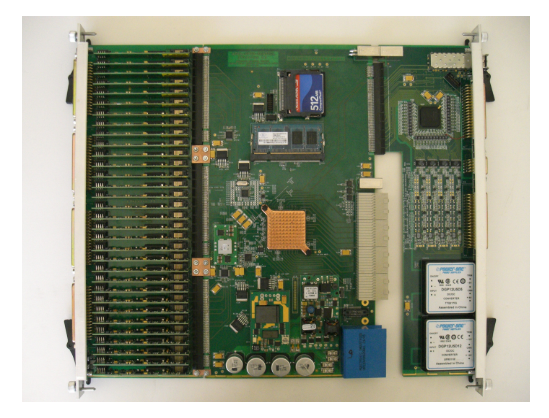
\includegraphics[width=0.5\textwidth]{Chp2/PCIboard.png}
	\caption{\label{PCIe}  ATCA control board with 32 ADCs developed and assembled  at the IPFN. \cite{ATCA2010}}
	
\end{figure}

\begin{figure}[htbp]
	\centering
	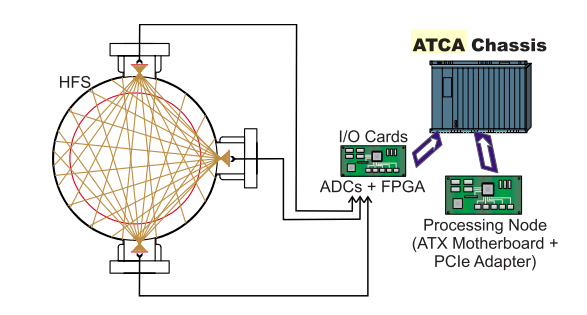
\includegraphics[width=0.55\textwidth]{Chp2/Tomogr.png}
	\caption{\label{Tomog}  The ISTTOK tomography system has 30 acquisition channels connected by an Input-Output ATCA card and processed using the MARTe framework.  \cite{Ivo_tomo}}
	
\end{figure}

For the Compass Tokamak ( Prague, Czech Republic), its whole control and data acquisition system was redesigned and built from scratch, based also on the ATCA standard. In total 14 ATCA  boards (developed at IPFN) will be used with 32 ADCs each one. In order to guarantee real-time execution of the control codes a framework based on Linux and the Real-Time Application Interface (RTAI) will be used. This will explore the features provided by the new multi-core technologies \cite{ATCA2010}. Figure  ~\ref{Compass} shows an schematic of the new COMPASS system.
\smallskip


\begin{figure}[htbp]
	\centering
	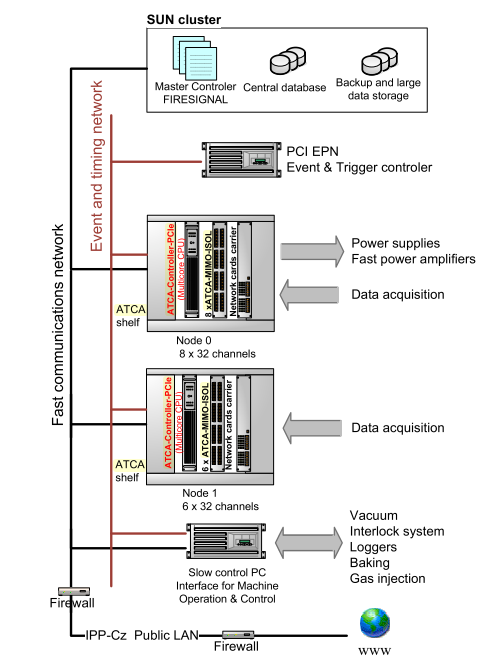
\includegraphics[width=0.55\textwidth]{Chp2/COMPASS_ATCA.png}
	\caption{\label{Compass} Schematic of COMPASS tokamak control and data acquisition
		system,  two ATCA systems are responsible for the fast control of the device and for the data acquisition. \cite{ATCA2010}}
	
\end{figure}

\subsection{MARTe 2.0}
Software Quality Assurance (QA)\footnote{Software QA is a set of activities or processes that define and assess the adequacy of software processes to provide evidence that establishes confidence that the software processes are appropriate for and produce software products of suitable quality for their intended purposes~\cite[Chapter 5.1]{SQA}.} processes are being applied to the development of a new version of the MARTe framework also  called MARTe 2.0. The  main objective is to provide a QA certifiable environment from where it is possible to develop, with less effort, certifiable applications. The  MARTe QA version can be easily adapted to the development of many types of software which are common in the fusion community, in particular for software related to control and data acquisition systems that is to be shared among different teams  ~\cite{MARTe2}. MARTe 2.0 will be the result of reduction exercise of the core framework based on the lessons learned from MARTe. This version will incorporate and implement an integral quality assurance process for the development of the framework (e.g. unit tests and coding standard) ~\cite{MARTe2PMP}. 
\smallskip

In order to develop robust code and to avoid common errors and pitfalls, a controlled subset of the C++ language must be defined for the MARTe framework. This subset will be defined by means of a list of coding rules, which will address all dangerous aspects of the C++ language for critical systems \footnote{This list of coding rules has as one of the main objectives to identify potentially dangers associated  with type conversions like loss of value, loss of sign and loss of precision ~\cite{MISRA2008}. }. Thus, the C++ version used on MARTe will be defined by the standard ISO/IEC 14882:2003 aka as C++03, while the coding rules will be those defined by the standard MISRA C++:2008 ~\cite{MARTe2Code}. The MARTe project manager is responsible for appointing a quality office (QO) for the QA process. The QO will guarantee that the QA activities are executed accordingly to the software development process, it will also conduct independent reviews and audit all data and processes involving the development, production and maintenance of MARTe deliverables ~\cite{MARTe2QAP}. The overall advantage of the new MARTe version is that the common faced difficulties of distributing and maintaining a software without  the continuous support of the original developers will be overcome following a complete QA system.



\section{Plasma equilibrium codes} 

Tokamak equilibrium codes are used for retrieving information about plasma current, shape and position and pressures profiles among other parameters. Usually these codes use as input data as the machine geometry, the PF coils currents and the flux and magnetic field diagnostics measurements. The importance of these codes is that since some of the parameters necessary for an accurate feedback control are not directly measured from the diagnostics,  this data has to be fitted on real-time somehow to the Grad-Shafranov equilibrium model~\cite{Shafranov1971}. In this section some of the most implemented and reported codes for tokamak plasma equilibrium reconstruction will be briefly  described.
\smallskip 


The EFIT (Equilibrium Fitting) code is used to efficiently reconstruct the current profile parameters, the plasma shape  and a current density profile satisfying the MHD equilibrium constraint  based on a Picard iteration\footnote{Picard iterations is a method based on  successive approximations to obtain a set of conditions under which an initial value problem has a unique solution.} approach which approximately conserves the external magnetic measurements ~\cite{EFIT1985}. EFIT has served as the de-facto standard technique to infer equilibrium from experimental diagnostics and there have been many different code implementations of this technique, all EFIT versions  are able to solve the MHD force balance and most experiment-specific customizations are made for the addition of experimental constraints peculiar to the experiment being modelled~\cite{EFIT2013}. EFIT reconstruction code is used in tokamaks such as DIII-D and the National Spherical Torus Experiment (NSTX). For the specific NSTX case they implemented a special real-time EFIT version called rtEFIT developed at General Atomics, the rtEFIT code provides the shape of the plasma boundary that is used as input to an isoflux control algorithm that generates voltage requests to the power supplies. The reconstruction of plasma boundaries  in real-time compare well to those reconstructed using the EFIT code offline in between plasma discharges ~\cite{rtEFIT}.
\smallskip


The RAPTOR (RApid Plasma Transport simulatOR)  is a model-based control-oriented code that predicts tokamak plasma profile evolution in real-time, it predicts the evolutions of several parameters, thanks to its accurate yet simplified physics model \cite{Raptor}. The physical model of the plant is derived from a spatially discretized partial differential equation (PDE), yielding a nonlinear set of ordinary differential equations (ODEs) for which the derivatives are evaluated analytically by the RAPTOR code. One of the main RAPTOR features is that  while the plasma is evolving RAPTOR has full knowledge of the plasma profiles and the available real-time diagnostic data can be included in a natural way to improve the accuracy of the estimation, in control engineering this approach is known as dynamic state observer and is used to estimate unmeasured or  poorly states of a dynamical system ~\cite{RAPTOR2011}. This dynamic state observer consists on an extended Kalman filter which estimates an augmented state consisting of physical states and random-walk disturbances  ~\cite{RAPTOR2014}. The concepts of  states-space systems and Kalman filtering will be addressed in the next subsections.  Figure ~\ref{RaptorMARTe} scheme shows  the  integration of the RAPTOR code on top of the MARTe framework at the Italian tokamak RFX-mod.
\smallskip

\begin{figure}[htbp]
	\centering
	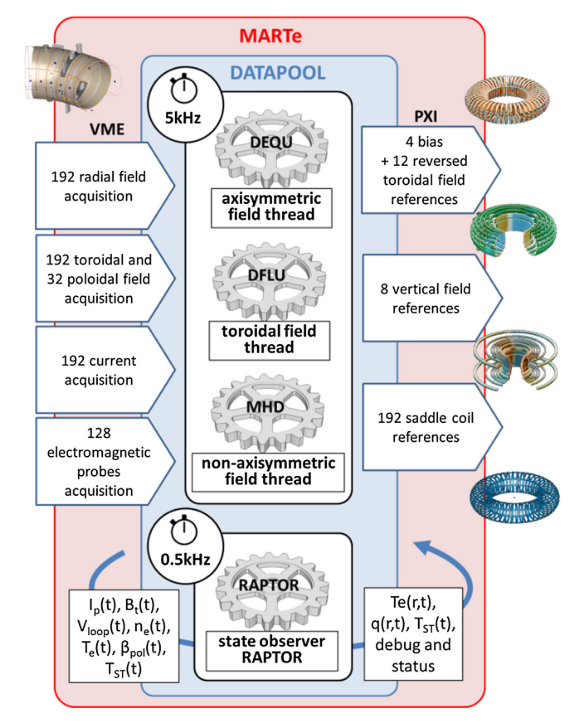
\includegraphics[width=0.505\textwidth]{Chp2/raptorMARTe.png}
	\caption{\label{RaptorMARTe} Skectch of the integration of the state observer RAPTOR in the RFX-mod real-time control system based on the MARTe framework.
		experimental \cite{Raptor}}
	
\end{figure}

For the case of JET  a  boundary reconstruction package called XLOC has been used to identify the X-point position and plasma boundary ~\cite{xloc}.  A newer code relying on XLOC  called Equinox was designed and implemented in C++ using a finite element method and a non linear fixed point algorithm associated to a least  square optimization procedure to reconstruct the plasma equilibrium in less than 50ms for the real-system~\cite{equinox}. 
\smallskip


The CREATE  codes (CREATE-L~\cite{Albanese:CREATEL} and CREATE-NL~\cite{Albanese:CREATENL}) are  equilibrium solvers which are widely described in next chapter as well as their application to plasma shape and position control design for the JT-60SA tokamak.
 


\section{Control Techniques and State-Space models}

This section will summarize  some systems dynamics and control  concepts which will be applied on the next chapters.\smallskip

 Applying a feedback control loop to a system  brings a link between the output and input signals, this action corrects the error in between the system output and a desired set-point,  eventually  the objective  of any closed loop controller is to take and maintain  the output signal at a prescribed value. The reduction of the system error is merely one of the many important effects that feedback may have upon a system, that is the reason why this sections will deepen in several control techniques ~\cite[Chapter~1]{Golnaraghi2010}. This section will also delve into the state-space models concepts since it will be a recurrent representation  for several systems presented in next chapters.

\smallskip

\subsection{State-Space models}
\label{SS_subsec}
State-space models are  crucial for the overall development of the work presented on this thesis whether they are used to describe a tokamak linear model for plasma position and  shape control or used to model some other relevant variables.  The first concepts  to be summarized on this section are the state variable and state equation definitions (\cite[Chapter~10]{Golnaraghi2010}, ~\cite[Chapter~2]{Kailath1980}).   \smallskip

Let the $n$ state equations of $nth$-order dynamic system be represented as:

\begin{equation}
	\frac{dx_i (t)}{dt} ~ = ~ f_i [x_1(t),x_2(t),...,x_n(t), u_1(t),u_2(t),...,u_p(t),w_1(t)w_2(t),...,w_v(t)]
	\label{stateEqs}
\end{equation}

 where $i=1,2,..,n$. The $ith$ state variable is represented by $x_i(t)$; $u_j(t)$ denotes the $jth$ input for $j=1,2,..,p$; and $w_k(t)$ denotes the $kth$ disturbance\footnote{The unknown disturbances acting on the state-space model are assumed to be generated by independent stochastic noise vectors. } input, with $k=1,2,..,v~$.\smallskip
 
 Let $y_1(t),y_2(t),...,y_q(t) $ be the q system output variables. The output variables are functions of the state variables  and the input variables. The output equations can be expressed as:
 \begin{equation}
 	y_j(t)=g_j[x_1(t),x_2(t),...,x_n(t),u_1(t),u_2(t),..,u_p(t),w_1(t)w_2(t),...,w_v(t)]
 \label{outputEq}
 \end{equation}
 
 where $j=1,2,..,q$~.
 \smallskip
 
 The set of $n$ state equations from ~\ref{stateEqs} and the $q$ output equations in ~\ref{outputEq} together they form the \textit{dynamic equations}. In order to have an easier form of expression and manipulations of these equations is common to represent them in vectors and matrices as follows: \smallskip
 
 \textbf{State vector:}
 \begin{equation}
 x(t)=
 \left[
 	\begin{matrix}
 	x_1(t)\\
 	x_2(t)\\
 	\vdots\\
 	x_n(t)
 	\end{matrix}
 	\right] 
 \end{equation}
 
\textbf{ Input vector:}
 
  \begin{equation}
 u(t)=
 \left[
 \begin{matrix}
 u_1(t)\\
 u_2(t)\\
 \vdots\\
 u_p(t)
 \end{matrix}
 \right] 
 \end{equation}
 
 \textbf{ Output vector:}
 
   \begin{equation}
y(t)=
 \left[
 \begin{matrix}
 y_1(t)\\
 y_2(t)\\
 \vdots\\
 y_q(t)
 \end{matrix}
 \right] 
 \end{equation}
 
\textbf{ Disturbance vector:}
    \begin{equation}
 w(t)=
 \left[
 \begin{matrix}
 w_1(t)\\
 w_2(t)\\
 \vdots\\
 w_v(t)
 \end{matrix}
 \right] 
 \end{equation}
 
 Using these defined vectors, equation ~\ref{stateEqs} can be written for the $n$ states like:\smallskip
 
 \begin{equation}
 	\frac{dx(t)}{dt}~=~ f[x(t),u(t),w(t)]
 \end{equation} 
 where f is a vector containing the functions $f_1,f_2,..,f_n$ as elements. In the same way the equations from ~\ref{outputEq} become:
 \begin{equation}
 	y(t)=g[x(t),u(t),w(t)]
 \end{equation}
 where $g$ is a vector containing the functions $g_1,g_2,..,g_n$ as elements.
 
 For a system that is time-invariant and linear like the ones shown on next chapter, the equations can be re-writen as:
 
 \begin{align}
	\frac{dx(t)}{dt}~=~ Ax(t)~+~Bu(t)~+Ew(t) \\
	y(t)=Cx(t)+Du(t)+Hw(t)
 \end{align}

  where $A$ is the state matrix, $B$ is the input matrix, $C$ is the output matrix, $D$ is the feed-forward matrix and  $E$ and $H$ are disturbances matrices. For simplification is usual the study of state-space and controllers concepts under the assumption that $w(t) =0$ which leads to the form:
 \smallskip
 \begin{align}
 	 \frac{dx(t)}{dt}~=~ Ax(t)~+~Bu(t)\\
 	  y(t)=Cx(t)+Du(t)
 	  \label{SS_eqs}
 \end{align}

 When applying the Laplace transform to system from ~\ref{SS_eqs} it leads to:
 \begin{align}
 	x(s)=(sI-A)^{-1}[x(0)+Bu(s)]\\
 	y(s)=C(sI-A)^{-1}[x(0)+Bu(s)]+Du(s)
 	\label{SS_eqs_lap}
 \end{align}
 
 where $x(0) $is the initial state or initial conditions from the system~\cite[Chapter ~4]{Chen1999}. The representation of the system from equation ~\ref{SS_eqs_lap} will be used in next subsections.\smallskip
 
State-space dynamics can describe Multiple-Input Multiple-Output (MIMO) models where a number of inputs $n_{~inputs}>~1$ can relate through the dynamics  matrices of the system to a number of outputs $n_{~outputs}>~1$. Given the physical conditions of the systems that will be analyzed and controlled in this work MIMO models will show several times.


\subsection{PID control}
\label{PID_sec}
This subsection will shortly address the Proportional-Integral-Derivative (PID) control  concepts. PID controllers are presently the most common ones in industrial applications and they are used several times through all this work. The PID controller has three parameters; proportional gain, integral gain, and derivative gain, they have proved through the years to provide a suitable control for a variety of systems despite not being optimal always. The usefulness of PID controls lies in their general applicability to most control systems. In particular, when the mathematical model of the plant is not known and therefore analytical design methods cannot be used, PID controls prove to be most useful.  
\smallskip

The closed-loop systems compensate the disturbances by measuring the output
response, feeding that measurement back through a feedback path, and comparing
that response to a reference or set point. If there is any difference between
the two signals, the system drives the plant, via the actuating signal, to make a
correction. If there is no difference, the system does not drive the plant, since the
plant’s response is already the desired set point ~\cite[Chapter ~1]{Nise}. Closed-loop systems also focus on achieving the stability as a system must be stable in order to produce the proper transient and steady-state response~\cite[Chapter ~3]{Nise}, thus if the closed-loop system poles are in the left half of the plane the feed-back system will be stable.
\smallskip

Systems that feed the error forward to the plant are called proportional control systems. Systems that feed the integral of the error to the plant are called integral control systems. Finally, systems that feed the derivative of the error to the plant are called derivative control systems~\cite[Chapter ~9]{Nise}. A PID controller consists on a feedback control loop where the current, previous and future error signal  between the output of the system and a given set point, is multiplied by the PID gains  and then sumed converting this signal into the system input, the effects on the feedback loop from each one of the gains will be described.

 When the model of the system plant is known it is possible to apply designing techniques for the PID gains like the Ziegler-Nichols method. When is not the case analytical or even intuition arising from the physics and numerics of the problem should be applied. Figure ~\ref{PID_scheme} shows the block scheme of a PID controller with a system plant $G(s)$ on the Laplace domain.

\begin{figure}[h]
	\centering
	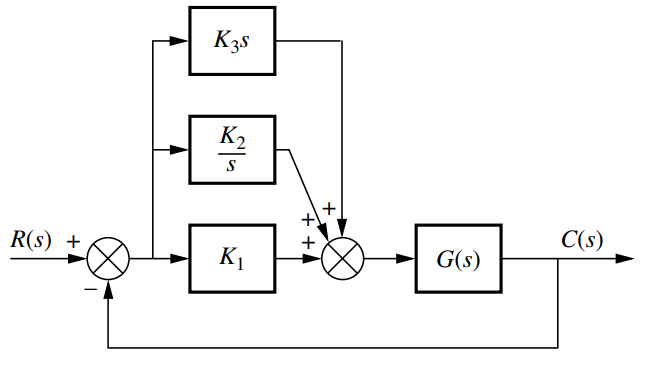
\includegraphics[width=0.55\textwidth]{Chp2/PID_scheme.png}
	\caption{ Plant and PID controller block scheme on Laplace domain ~\cite[Chapter~ 9]{Nise}. \label{PID_scheme}}
\end{figure}

 An only  proportional controller   relates the output of the system to the input by a proportional constant, and even though it performs a first approach to follow the  set point and stabilizes,  it results in a steady-state error or offset, such error may be eliminated with integral control action, see figure ~\ref{propGain}.
\smallskip

\begin{figure}[h]
	\centering
		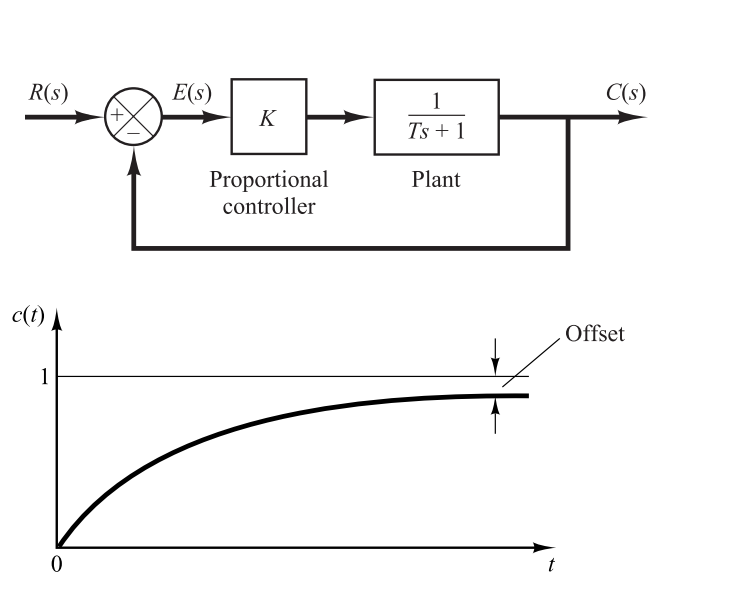
\includegraphics[width=0.55\textwidth]{Chp2/propgain.png}
	\caption{ Plant with a proportional (P) control  scheme on the Laplace domain and its response to a unit-step. The offset or error between the steady-sate response is also pointed out~\cite[Chapter~ 5]{Ogata2009}. \label{propGain}}
\end{figure}


The integral gain produces a signal that is proportional to the time integral of the error system, the offset or steady-state error can be eliminated by the sum of an integral action, the integral term also tends to produce and oscillatory response. This is an  important improvement over the proportional control alone, which gives an offset. Since the PI controller is also a low-pass filter, it helps filtering out the high-frequency noise  ~\cite[Chapter ~9]{Golnaraghi2010}, ~\cite[Chapter~ 5]{Ogata2009}. Figure ~\ref{PI} shows the block scheme of a PI controller and its response to a unitary step.
\smallskip

\begin{figure}[h]
	\centering
	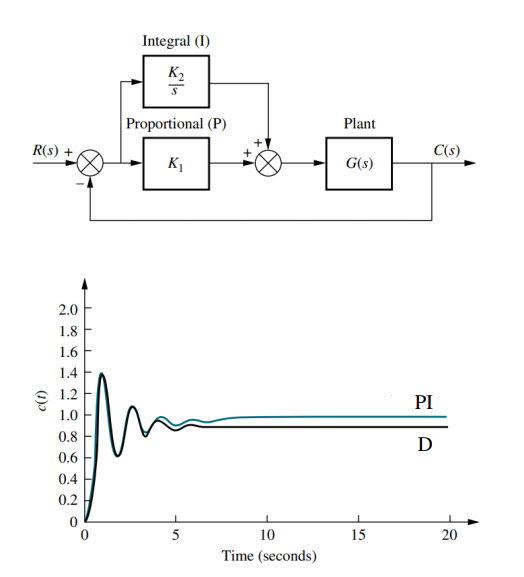
\includegraphics[width=0.55\textwidth]{Chp2/PI_Dcomp.png}
	\caption{  Plant scheme of   a plant with  a proportional-integral (PI) control   on the Laplace domain. Bottom graph corresponds to a step response to closed-loop systems with D and a PI controller ~\cite[Chapter~ 9]{Nise}, a visible improvement on the state-state error with the PI control is observable.  \label{PI}}
\end{figure}

The derivative gain added to a proportional controller gives a more sensitive controller which responds to the rate of change of the error and can produce a significant correction before the magnitude of the error becomes to large. In general, derivative control anticipates the actuating error, adds damping  and tends to increase the system stability, figure~\ref{propderGain} depicts the scheme and system response with a PD controller. The PD control uses the error derivative ~$de(t)/dt$ which allows the control to anticipate the error direction, it initiates an early corrective action which means an improvement on the transient response   ~\cite[Chapter ~9]{Golnaraghi2010},~\cite[Chapter ~9]{Nise}. Normally in linear systems when the slope of $e(t)$ is large overshoots may occur, when using a PD controller it also corrects the overshoot. 
\smallskip

\begin{figure}[h]
	\centering
	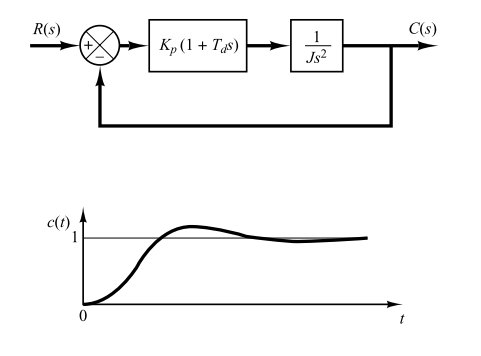
\includegraphics[width=0.55\textwidth]{Chp2/propderivgain.png}
	\caption{ The top scheme shows a PD controller for a  plant that is only modeled as an inertial load, on the graph below is shown the system response where it is possible to observe an offset reduction and a controlled transient as compared with the P controller ~\cite[Chapter~ 5]{Ogata2009}. \label{propderGain}}
\end{figure}

A PID controller improves the steady-state error and the transient response. Figure ~\ref{PID} shows the response time traces  of the same system with a PID, PD and D controllers to a unit step.
\smallskip



\begin{figure}[h]
	\centering
	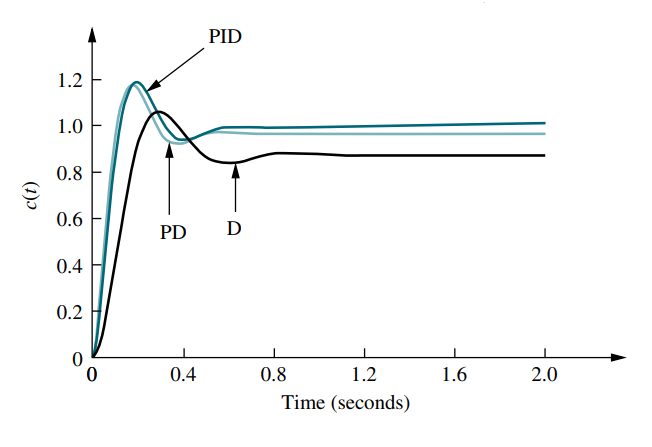
\includegraphics[width=0.505\textwidth]{Chp2/PID_comp.png}
	\caption{ Step response to closed-loop systems with D, PD and PID controllers ~\cite[Chapter~ 9]{Nise}. \label{PID}}
\end{figure}

\subsection{Multiple-Input Multiple-Output control}
\label{MIMO_sec}
This subsection will discuss the pole-place method and the linear quadratic optimal regulator (LQR) for control systems in state-space already discussed in subsection~\ref{SS_subsec}.  State feedback controllers basically relocate the eigenvalues of the given system through a state-feedback multiplication by a constant gain matrix $K$ so the system can follow a reference and be stabilized if necessary.
 \smallskip
 
 The concept of pole should be introduced as it will be related to  the definitions of the MIMO control methods. The poles $p_i$ of state-space system are the eigenvalues $\lambda_i(A),~i=1,..,n$ of the system matrix $A$. Poles are important for establishing the stability of a system, for continuous systems a linear dynamic system  $	\dot{x}(t)~=Ax(t)+Bu(t)$ , where $\dot{x}(t)$ stands for $dx/dt$, is stable if and only if all poles are in the open left half plane (LHP), that is $\mathbb{R}e~{\lambda_i(A)}<~0, \forall i$. Eigenvalues in the right half plane(RHP) with  $\mathbb{R}e~{\lambda_i(A)}\geq~0$ give raise to unstable modes since for this case $e^{\lambda_i(A)~t}$ is unbounded as $t\rightarrow~\infty$,  eigenvalues in the open LHP give raise to stable modes where $\mathbb{R}e~{\lambda_i(A)} \rightarrow 0$ as $t\rightarrow~\infty$~\cite[Chapter~4]{Skogestad}.
\smallskip

Consider the system:
\begin{align} 
	\dot{x}(t)~=Ax(t)+Bu(t) 	\label{SS_eq}\\
y(t)=Cx(t) \nonumber
\end{align}

where it is assumed that $D=0$. In state feedback, the input $u(t)$ is given by:

\begin{equation}
	u(t)=r(t)-Kx(t) = r(t)-[k_1~ k_2~\cdots ~k_n] x(t)=r-\sum_{i=1}^{n}~k_ix_i
	\label{u(t)}
\end{equation}

as shown in figure~\ref{SS_schm}. Each feedback gain $k_i$ is a real constant.This is called the constant gain negative state feedback or in a simpler form \textit{state feedback}~\cite{Chen1999}. Substituting equation ~\ref{SS_eq} into ~\ref{u(t)} its obtained:
\begin{align} 
\dot{x}(t)~=(A-B~K)x(t)+Br(t) \label{SS_eq_feed} \\
y(t)=Cx(t) \nonumber
\end{align}



\begin{figure}[h]
	\centering
	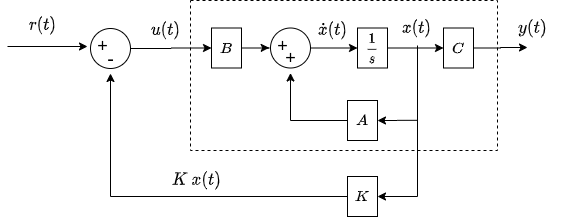
\includegraphics[width=0.6\textwidth]{Chp2/SS_scheme.png}
	\caption{  State-space model with a $K$ gain matrix feedback scheme.\label{SS_schm}}
\end{figure}


The first control MIMO algorithm to be addressed  is the pole-placement method which consists in placing the closed-loop system poles in certain location by means of state feedback through an appropriate state feedback gain matrix $K$, the design objective of the pole-placement design is to find  $K$ such that the eigenvalues or poles of $(A-BK)$, or the closed-loop system, are of certain prescribed values. For this method the eigenvalues of the closed-loop system can be assigned arbitrarily  as long as they are stable~\cite[Chapter~10]{Golnaraghi2010}. The  determination of the desired closed-loop poles is based on the transient-response and/or frequency-response requirements, such as speed, damping ratio, or bandwidth, as well as steady-state requirements ~\cite[Chapter~10]{Ogata2009}.
\smallskip

Let's consider the system given in equation ~\ref{SS_eq_feed} and the feedback control input from ~\ref{u(t)}, by substituting one on the other the closed-loop system is represented by the equation:
\begin{equation}
	\dot{x}(t)=(A-BK)x(t) + Br(t)	\quad ,
\end{equation}

 $K$ is the $1\times n$ feedback matrix that can give an arbitrary set of eigenvalues or poles of $(A-BK)$, which are the $n$ roots of the Laplace equation~\cite[Chapter~10]{Golnaraghi2010}:
\begin{equation}
	|sI-A+BK|=0 \quad.
\end{equation}

 From the canonical representation of equation ~\ref{SS_eq} its obtained (~\cite[Chapter~10]{Golnaraghi2010}, ~\cite[Chapter~4]{Chen1999} ) :
 \begin{align}
 A=\begin{bmatrix}
 0& 1& 0 & \cdots & 0\\
 0 & 0 & 1 & \cdots & 0\\
 \vdots & \vdots & \vdots &\ddots & \vdots \\
 0 & 0 & 0 & \cdots & 1 \\
 -a_0 & -a_1 & -a_2 & \cdots & -a_{n-1}
 \end{bmatrix} \quad
 B=\begin{bmatrix}
 0 \\ 0 \\ \vdots \\ 0 \\ 1
 \end{bmatrix} \quad .
 \end{align}

Then the gain feedback matrix $K$ is expressed as:
\begin{equation}
K= [k_1~k_2~\cdots ~ k_n]
\end{equation}
 where ~ $k_1,k_2,\cdots,k_n$ are real constants, this leads to the expression:
 
 \begin{equation}
 A-BK=\begin{bmatrix}
 0& 1& 0 & \cdots & 0\\
 0 & 0 & 1 & \cdots & 0\\
 \vdots & \vdots & \vdots &\ddots & \vdots \\
 0 & 0 & 0 & \cdots & 1 \\
  -a_0-k_1 & -a_1-k_2 & -a_2-k_3 & \cdots & -a_{n-1}-k_n
 \end{bmatrix}
 \end{equation}
 
 The eigenvalues or poles of $A-BK$ can be found from the characteristic equation:
 
 \begin{equation}
 |sI-A+BK|=s^n +(a_{n-1}+k_n)s^{n-1}+(a_{n-2}+k_{n-1})s^{n-2}+ \cdots + (a_0+k_1) =0
 \end{equation}
 
 \noindent since the elements $k_1,k_2,\cdots,k_n$ are isolated in each coefficient of the characteristic equation the eigenvalues can be arbitrarily assigned to any set of stable poles ~\cite[Chapter~10]{Golnaraghi2010},~\cite[Chapter~10]{Ogata2009}.\smallskip
 
%% LQR
Another control technique for state-space feedback is the optimal control refereed as  Linear Quadratic Gaussian (LQG) or Linear Quadratic Regulator (LQR). It is assumed that the plant dynamics are linear and there are noise measurements and disturbance signals stochastic with known statistical properties ~\cite[Chapter~9]{Skogestad}.

Consider the system:
\begin{equation}
	\dot{x}(t)~=Ax(t)+Bu(t)
\end{equation} 

\noindent that has an initial condition $x(t_0)=x_0\neq 0$. Therefore $x(t) \neq 0~,t\geq ~t_0$ and the regulator problem is to apply an  input signal $u(t)$ that takes the system back to the zero state in an optimal manner. The manner the LQR regulator achieves this is by minimizing the deterministic cost~\cite[Chapter~9]{Skogestad},\cite[Chapter~3]{Golnaraghi2010}:
\begin{equation}
J_r=\int_{0}^{\infty}(x(t)^T~Q~x(t)~+~ u(t)^T~R~u(t)dt 
\end{equation}

\noindent where $Q$ is a positive-definite Hermitian or real symmetric matrix and $R$ is a positive-definite Hermitian or real symmetric matrix. The optimal solution is for any initial state $u(t)=-K_rx(t)$ where:
\begin{equation}
K_r=R^{-1}~B^T~X
\label{K_optim}
\end{equation}

and $X=X^T~\geq 0$ is the unique positive-semidefinite solutions of the algebraic Ricatti equation
\begin{equation}
A^TX~+~XA~-~XBR^{-1}B^TX~+Q=0\quad.
\label{Ricatti}
\end{equation}

In order to design the optimal $K_r$ feedback gain the Ricatti equation ~\ref{Ricatti} has to be solved for the matrix $X$ and then substitute into equation ~\ref{K_optim}.


\subsection{Observers and Kalman filters}

In practical real systems that have been modeled as state-space  it may occur that the state vector, which is vital for performing the feedback control of the methods just presented, is not fully measurable, when this occurs is necessary to retrieve the state vector $x(t)$ from the  system outputs $y(t)$ and  is obtained through an state estimator also called observer to estimate not measurable state variables ~\cite[Chapter~8]{Chen1999}. A state observer estimates the state vector based on the measurements of the output  and inputs system signals. The inputs of the observer are the output $y(t)$ and the control input $u(t)$. Similarly with the construction of a state-space controller, the observer uses an observer gain matrix $K_{obs}$ which is a weighting matrix to the correction term involving the difference between the measured output $y(t)$ and the estimated output $C~x_{est}(t)$, where $x_{est}(t)$ are the estimated states~\cite[Chapter~10]{Ogata2009}. 
\smallskip

Through the observer gain matrix $K_{obs}$ is possible to retrieve an estimated state-space model which will have as output the reconstructed states $x_{est}(t)$ and the reconstructed outputs $y_{est}(t)$, the estimation error or observation error is the difference between $y(t)$) and $y_{est}(t)$. Figure ~\ref{plant_obser} shows a scheme of state-space plant model and a observer block to reconstruct the states. 
\smallskip

\begin{figure}[h]
	\centering
	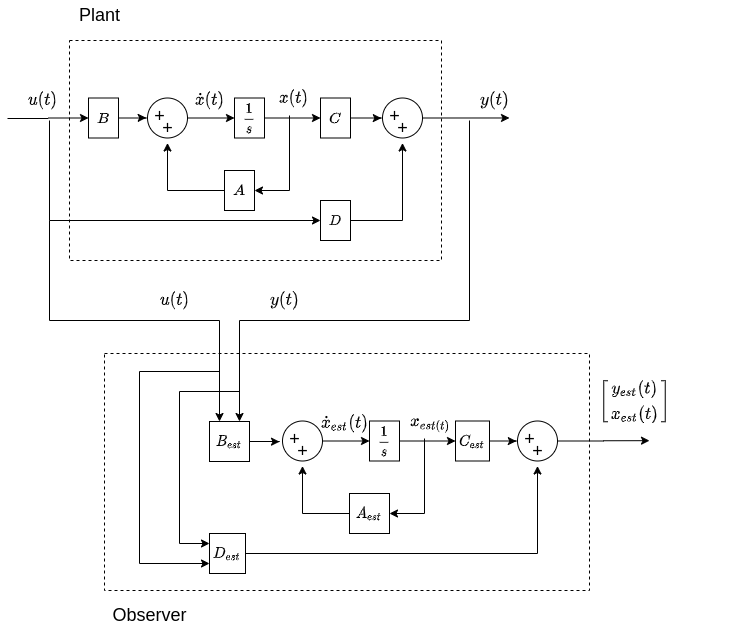
\includegraphics[width=0.7\textwidth]{Chp2/plant_observer.png}
	\caption{ Scheme of a state-space model plant and its observer or state estimator. \label{plant_obser}}
\end{figure}

Kalman filters have the structure of an ordinary state estimator but they take into account the process and measurement noise($\omega_d\,,\omega_n$) from the inputs signals. In Kalman filters the optimal choice of $K_{obs}$, which minimizes  the covariance $E{[x-x_{est}]^T~[x-x_{est}]}$, is given by(~\cite[Chapter~9]{Skogestad},~\cite[Chapter~8]{Hippe2009}):  

\begin{equation}
K_{obs}=Y~C^T~V^{-1}
\label{K_obs}
\end{equation}
 where $Y=Y{ T}~ \geq 0$ is the unique positive-semidefinite solution of the algebraic Ricatti equation:
 
 
\begin{equation}
YA^T~+~AY~-~YC^TV^{-1}CY~+W=0
\label{Ricatti2}
\end{equation}

where $W$ is a positive-definite Hermitian or real symmetric matrix and $V$ is a positive-definite Hermitian or real symmetric matrix, solving equation ~\ref{Ricatti2} for Y and substituting on ~\ref{K_obs}, gives the optimal $K_{obs}$ for reconstructing the states of the original system. The combination of an optimal state estimator or Kalman filter  and an optimal state feedback or LQR controller is commonly called LQG, this type of compensator-estimator configuration will be used ahead for implementation of plasma position controllers. 

\subsection{Experimental identification of state-space models}
\label{data_drivenSec}
When experimental work is carried out most of the times the available signals are not continuous. In addition it may happen that a theoretical model  linking experimental signals as inputs and outputs of it does not exist or has not been modeled yet. This section will address the representation in discrete time of state-space models as well as a method for retrieving a model based on experimental data  along with some useful concepts.
\smallskip

For some physical systems it is natural to work with the continuous-time representation of the systems since most of the basic relationships are expressed in terms of differential equations. The relation between the Laplace transform of the input and output of the system  is called \textit{transfer function} and is represented as $Y(s)=G_C(s)U(s)$, where introducing $p$ as the differential operator the time-domain transfer function yields as:  $y(t)=G_C(p)u(t)$. Taking into account the disturbances that influence  the system the transfer function can be re-written as: $y(t)=G_C(p)u(t)+H(q)w(p)$ ~\cite[Chapter~2]{Ljung1987}. Thus, the discrete transfer function will be $G_C(p) \rightarrow ~G_T(q)$  where $q$ is the discrete time shift operator, for the state-space models variables $G_T$ and $H$ are matrices. The concept of transfer function will be frequently used in this section.
\smallskip


\subsubsection{State-Space discrete models}
When implementing numerical methods and models in digital computers it is necessary to transfer the continuous variables and models to their discrete equivalents. If an input $u(t)$ is generated by a digital computer followed by a digital to analog converter (DAC), then $u(t)$ will be piecewise constant, this situation often arises in computer control of control systems~\cite[Chapter~4]{Chen1999}. Let:
\begin{equation}
u(t)=u(kT)=:u[k] \qquad for\: kT\leq~t~<(k+1)T
\end{equation}
for $k=0,1,2,..$, where $T$ is the sampling time. This input $u[k]$ changes values only at discrete time instants. If an input changes its value only at discrete time instants $kT$ and the response is only computed at $t=kT$ then discrete state-space model (considering absence of disturbances ) can be represented as:


 \begin{align}
x[k+1]=A_d[k]~+~B_du[k]\\
y[k]=C_dx[k]~+~D_du[k]
\label{SS_dscrt}
\end{align}
with
\begin{equation}
A_d=e^{AT}\qquad B_d=\left(\int_{0}^{T} e^{A\tau}d\tau\right)B \qquad C_d=C \qquad D_d=D \, .
\end{equation}



\subsubsection{Discrete state-space model identification}
\label{Disc_SS_ident}
For system identification purposes it is often desirable to use parametric models, i.e., a set of models is described by a number of real-valued parameters collected in a parameter  vector $\theta\in \mathbb{R}^d$ to be determined. A particular model is then represented by a value of the d-dimensional unknown parameters vector $\theta$ ~\cite[Chapter~2]{McKelvey1995}. Let's write the state-space model structure considering the discrete disturbances $w[k]$ in the form:

\begin{equation}
\mathcal{M}:\quad
\begin{aligned}
\hat{x}[k+1]&= A(\theta)\hat{x}[k] + B(\theta)u[k] + E(\theta)w[k] \\
y[k]&=C(\theta)\hat{x}[k]+w[k]
\end{aligned}
\label{M:}
\end{equation}

\noindent where  the vectors $\hat{x}$ and $\hat{y}$ are called predictors and they are the conditional expectations of $x(t)$ and $y(t)$ given information up to $k-1$ and the matrices A,B,C and E are constructed from the parameter vector $\theta$ according to the model structure $\mathcal{M}$. Let:

\begin{equation}
d_{\mathcal{M}}=dim ~\theta
\end{equation}
 denote the dimension of the parameter vector $\theta$ and let $\mathcal{M}(\theta)$ denote the model from equation ~\ref{M:}. The way of representing the disturbances in ~\ref{M:} is called the innovations form. The model will thus have the transfer functions:
 \begin{equation}
 G(q,\theta)=C(\theta)[qI-A(\theta)]^{-1}B(\theta)
 \end{equation}
 and
 \begin{equation}
 H(q,\theta)=I+C(\theta)[qI-A(\theta)]^{-1}K(\theta) \quad .
 \end{equation}

From equation ~\ref{M:}, the state predictor $\hat{x}[k+1]$ is given by:

\begin{equation}
\label{predictor}
\begin{aligned}
\hat{x}[k+1]&=[A(\theta)-K(\theta)C(\theta)]\hat{x}[k]~+~B(\theta)u[k]~+~-K(\theta)y[k] \\
\hat{y}[k|\theta]&=C(\theta)\hat{x}[k]
\end{aligned}
\end{equation}
 where  $\hat{y}[k|\theta]$ denotes the conditional expectation of $y[k]$ given the parameter vector $\theta$ ~\cite[Chapter~3]{Ljung1987}, this is a one-step ahead prediction and is denote as $\hat{y}[k|\theta]$ to emphasize its dependence on the parameter vector $\theta$.\smallskip
 
The system identification technique  applied is based on the prediction error minimization (PEM) ~\cite[Chapter~7]{Ljung1987}, ~\cite[Chapter~3]{Ljung1987}. The standard setting can be described as: given the experimental data consisting of an input vector {u[k]} and an output vector {y[k] } by:

\begin{equation}
Z^N~= \{y[k],u[k]|k=1,...,N\}, 
\end{equation}
 
\noindent and a model structure $\mathcal{M}$ defining  a mapping from the parameter space $D_{\mathcal{M}}$ to the outputs predictor $\hat{y}(t|\theta)$, the objective is to find the value $\hat{\theta}$ which minimizes a criterion $V_N(\theta)$. This criterion is defined as:
 \begin{equation}
 V_N(\theta)=\frac{1}{N} \sum_{t=1}^{N}|\varepsilon[k,\theta]|^2,
 \label{V_N}
 \end{equation}
 
 where $|\cdot|$ is the Euclidian $l_2-norm$. The prediction error is the vector
 \begin{equation}
 \varepsilon(t,\theta)~=y[k]-\hat{y}[k|\theta]
 \end{equation}
 with the predictor $\hat{y}(t|\theta)$ given by the equation ~\ref{predictor}. The minimizing parameter vector is defined by:
 \begin{equation}
 \hat{\theta}_N=\argmin_{\theta \in D_\mathcal{M}}~V_N(\theta)
 \end{equation}
 
\noindent where "arg min" is the operator returning the argument which minimizes the function. The minimization of $V_N(\theta)$ given in equation ~\ref{V_N}  as well as the properties of the resulting estimation of the parameters vector $\hat{\theta}_N$ under varying assumptions on the model structure $\mathcal{M}$ and the experimental data set $Z^N$, has been formulated in the related literature and computationally implemented, such is the case of the \textit{System Identification Toolbox} from \textsc{Matlab}. This toolbox relies on the function called "pem" for computing the error minimization which returns an estimated state-space model given a data vector of input and output signals\cite[Chapter~4]{Toolbox}, the model is adjusted by optimizing the prediction error fit, it is possible to select the order of the model or use the "best" order given by the toolbox. Due to its adaptability and flexibility, this toolbox was used for retrieving data-driven models in several stages of the implementation of real-time control algorithms in ISTTOK.